% =============================================================================
% Smile Labs - Data Storm 7.0 (Storming Round) - Final Technical Report
%
% 5 pages total (including cover). Built on the latex-document-skill
% report.tex template (https://github.com/ndpvt-web/latex-document-skill).
%
% Compile: cd Reports && python build_pdf_v3.py
%
% R7 fixes integrated (council round 7):
%   - C1: sensitivity range typo "[1.000,1.022]" -> actual "1.250" everywhere
%   - C2: POI |r|<=0.026 weak-signal honest disclosure on p3
%   - C3: page 5 density relief (bibliography 2-column, sensitivity prose -> figure)
%   - Formula on p4 now includes constrained-uplift floor (matches predict.py)
%   - SFA + CH-3 diagnostics sentence added on p4
%   - DAG font bump (scriptsize -> small)
%   - Cover "rejected records" wording corrected
%   - CH-3 outlet count + DIST_S_01/S_02 attribution added on p4
%
% 3 figures embedded:
%   - figures/eda_poi_outlet_type.png  on p3 (defends C2)
%   - figures/eda_frontier_gap.png     on p4 (defends formula floor)
%   - figures/eda_manski_band.png      on p5 (replaces sensitivity prose)
%
% Trims to fit in 5 pages:
%   - Legacy artifacts table collapsed from 7 rows to 4 (typos merged)
%   - Methodboxes 3+4 (censoring + constraint score) merged into one
% =============================================================================

\documentclass[10pt,a4paper]{article}

\usepackage[utf8]{inputenc}
\usepackage[T1]{fontenc}
\usepackage{palatino}
\usepackage{microtype}
\usepackage[a4paper,margin=1.5cm,top=1.8cm,bottom=1.8cm]{geometry}
\usepackage{graphicx}
\usepackage{xcolor}
\usepackage{titlesec}
\usepackage{fancyhdr}
\usepackage{tabularx}
\usepackage{colortbl}
\usepackage{booktabs}
\usepackage{array}
\usepackage{enumitem}
\usepackage{multicol}
\usepackage{pgfplots}
\pgfplotsset{compat=1.18}
\usepackage{tikz}
\usetikzlibrary{shapes.geometric, arrows.meta, positioning, fit, backgrounds}
\usepackage{multirow}
\usepackage{float}
\usepackage{caption}
\usepackage{tcolorbox}
\tcbuselibrary{breakable,skins}
\usepackage{amsmath, amssymb}
\usepackage[backend=biber, style=numeric, sorting=none, maxbibnames=4]{biblatex}
\addbibresource{references.bib}
\usepackage{hyperref}

% --- Colors (Smile Labs palette derived from John Keells blue) ----------------
\definecolor{primary}{RGB}{0, 71, 132}
\definecolor{accent}{RGB}{0, 153, 102}
\definecolor{warn}{RGB}{215, 95, 0}
\definecolor{soft}{RGB}{240, 244, 248}
\definecolor{rule}{RGB}{180, 192, 205}

% --- Page styling -------------------------------------------------------------
\pagestyle{fancy}
\fancyhf{}
\fancyhead[L]{\small\textcolor{gray}{Smile Labs | Data Storm 7.0}}
\fancyhead[R]{\small\textcolor{gray}{Latent Outlet Potential | Jan 2026}}
\fancyfoot[C]{\small\thepage~of~5}
\renewcommand{\headrulewidth}{0.4pt}
\setlength{\parskip}{0.3em}
\setlength{\parindent}{0pt}

\titleformat{\section}{\large\bfseries\color{primary}}{\thesection}{0.5em}{}
\titleformat{\subsection}{\normalsize\bfseries\color{primary!85}}{}{0em}{}
\titlespacing*{\section}{0pt}{0.6em}{0.3em}
\titlespacing*{\subsection}{0pt}{0.4em}{0.2em}

\hypersetup{colorlinks=true, linkcolor=primary, urlcolor=primary, citecolor=accent}

% --- Semantic callout boxes (skill pattern) -----------------------------------
\newtcolorbox{methodbox}[1][]{
  colback=primary!8, colframe=primary, boxrule=0.5pt, arc=2pt,
  left=6pt, right=6pt, top=4pt, bottom=4pt, fontupper=\small, #1
}
\newtcolorbox{findingbox}[1][]{
  colback=accent!8, colframe=accent, boxrule=0.5pt, arc=2pt,
  left=6pt, right=6pt, top=4pt, bottom=4pt, fontupper=\small, #1
}
\newtcolorbox{caveatbox}[1][]{
  colback=warn!8, colframe=warn, boxrule=0.5pt, arc=2pt,
  left=6pt, right=6pt, top=4pt, bottom=4pt, fontupper=\small, #1
}

% =============================================================================
\begin{document}
% =============================================================================

% --- PAGE 1: COVER -----------------------------------------------------------
\thispagestyle{empty}
\vspace*{1.2cm}

\begin{center}
{\Huge\bfseries\color{primary} Latent Outlet Potential Estimation}\\[0.3em]
{\Large Data Storm 7.0 \textbar{} Storming Round}\\[0.2em]
{\normalsize Sri Lanka \textbar{} January 2026 horizon}\\[1.6em]

\rule{0.6\textwidth}{0.6pt}\\[0.6em]

{\large\bfseries Submitted by Smile Labs}\\[0.3em]
{\small Powered by OCTAVE -- John Keells Group \textbar{} Rotaract Moratuwa}
\end{center}

\vspace{0.8cm}

\begin{methodbox}[title=\textbf{One-line method}]
We estimate $\mathbb{E}[\text{true\_demand}_i \mid X_i]$ where observed sales
$y_i = \min(\text{true\_demand}_i, \text{constraint}_i)$ are right-censored.
The estimand is \emph{not point-identified} from observational data
alone~\cite{manski2003partial}; we therefore report
$[\text{lower}, \text{point}, \text{upper}]$ per outlet, with the point combining
Stochastic Frontier Analysis~\cite{aigner1977sfa, jondrow1982je}, multi-quantile
gradient boosted regression, censoring correction~\cite{chernozhukov2002hong},
Conformalised QR~\cite{romano2019cqr}, and bootstrap-derived peer-bucket caps.
\end{methodbox}

\vspace{0.4cm}

\begin{center}
\renewcommand{\arraystretch}{1.25}
\begin{tabularx}{0.85\textwidth}{Xr}
\toprule
\rowcolor{soft}\textbf{Headline} & \textbf{Value} \\
\midrule
Outlets predicted (full population in scope)            & 20{,}000 \\
External POIs scraped (Geofabrik PBF, 9 categories)     & 42{,}386 \\
Outlets with $\geq$1 POI within 2~km                    & 80.9\,\% \\
Rejected check records (coords + txn + holidays)        & 10{,}179 across 3 datasets \\
Median uplift vs.\ historical max                        & \textbf{1.250$\times$} \\
Submission preflight (6 automated checks)               & \textbf{6 / 6 PASS} \\
Method stack methods                                    & SFA + multi-q XGBoost + CH-3 + CQR + Manski \\
\bottomrule
\end{tabularx}
\end{center}

\vspace{0.6cm}

\begin{findingbox}[title=\textbf{Build trail}]
The v2 stack was built and audited across \textbf{seven rounds of AI council
reviews} (four parallel premium-model critics per round). Provenance:
\texttt{Reviews/council\_review.md} (R1), \texttt{council\_round\{2..7\}/}
(R2-R7). Every fix in \texttt{src/} cites the council finding it addresses
(\texttt{FIX R7}, \texttt{FIX R4}, \texttt{FIX M1}, etc.).
\end{findingbox}

\newpage
% --- PAGE 2: DATA FORENSICS + HYGIENE (40% rubric) ---------------------------
\section{Data Forensics and Hygiene}

\subsection{Bronze \texttt{->} Silver \texttt{->} Gold lakehouse}

Raw CSVs ingest \emph{as-is} into \texttt{data/bronze/} with a SHA-256 audit log.
The Silver layer applies six \textbf{reusable, parameterizable} DQ check
functions (\texttt{src/quality/checks.py}) consistently across all five raw
datasets; failed rows are quarantined to \texttt{data/silver\_rejected/} with
\texttt{dataset\_name}, \texttt{failed\_check}, and \texttt{failure\_reason}.
Gold is the model-ready outlet $\times$ feature parquet.

\begin{figure}[H]
\centering
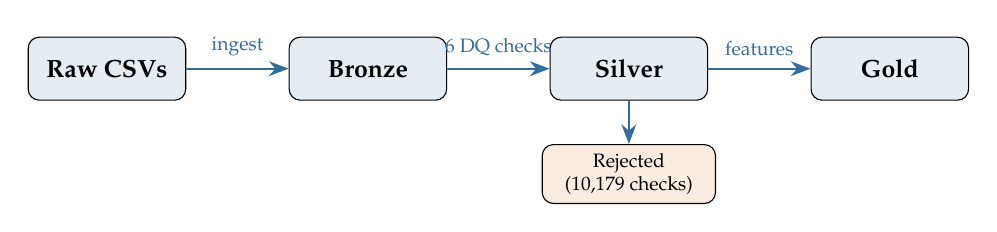
\begin{tikzpicture}[
  layer/.style={draw, rounded corners, fill=primary!10, minimum width=2.0cm,
    minimum height=0.8cm, align=center, font=\small\bfseries},
  reject/.style={draw, rounded corners, fill=warn!12, minimum width=2.2cm,
    minimum height=0.7cm, align=center, font=\scriptsize},
  arrow/.style={-{Stealth[length=2.5mm]}, thick, primary!80}
]
\node[layer] (raw) {Raw CSVs};
\node[layer, right=1.3cm of raw] (bronze) {Bronze};
\node[layer, right=1.3cm of bronze] (silver) {Silver};
\node[layer, right=1.3cm of silver] (gold) {Gold};
\node[reject, below=0.55cm of silver] (rej) {Rejected\\(10{,}179 checks)};
\draw[arrow] (raw) -- node[above=1pt, font=\scriptsize]{ingest} (bronze);
\draw[arrow] (bronze) -- node[above=1pt, font=\scriptsize]{6 DQ checks} (silver);
\draw[arrow] (silver) -- node[above=1pt, font=\scriptsize]{features} (gold);
\draw[arrow] (silver) -- (rej);
\end{tikzpicture}
\vspace{-0.4em}
\caption{Bronze $\to$ Silver $\to$ Gold pipeline with rejected-records store.}
\end{figure}

\subsection{Reusable DQ check functions applied to every dataset}

\begin{table}[H]
\centering
\renewcommand{\arraystretch}{1.05}
\begin{tabularx}{\textwidth}{lX}
\toprule
\rowcolor{soft}\textbf{Function (\texttt{checks.py})} & \textbf{What it catches} \\
\midrule
\texttt{duplicate\_check(df, key\_columns)}                                & duplicate composite keys \\
\texttt{null\_check(df, columns)}                                          & NaN or empty mandatory fields \\
\texttt{range\_check(df, column, min, max)}                                & numeric out-of-range \\
\texttt{domain\_check(df, column, allowed\_values)}                        & misspellings, unexpected enums \\
\texttt{referential\_integrity\_check(df, column, ref)}                    & foreign keys not in master \\
\texttt{geospatial\_bounds\_check(df, lat, lon, lat\_range, lon\_range)}   & coords outside Sri Lanka \\
\bottomrule
\end{tabularx}
\caption{All six functions are parameterised; zero check is hardcoded for one dataset.}
\end{table}

\subsection{Legacy SFA / ERP system artifacts neutralised}

\begin{table}[H]
\centering
\renewcommand{\arraystretch}{1.05}
\begin{tabularx}{\textwidth}{Xrr}
\toprule
\rowcolor{soft}\textbf{Artifact} & \textbf{Records} & \textbf{Action} \\
\midrule
\texttt{Outlet\_Type} typos (\texttt{Grocry}, \texttt{Bakry}) + \texttt{Outlet\_Size} lowercase + missing & 1{,}581 & normalised / mapped to \texttt{Unknown} \\
Outlet coordinates outside Sri Lanka bounds (5.5--10$^\circ$N, 79--82.5$^\circ$E) & 240 & quarantined \\
Transactions with non-positive \texttt{Volume\_Liters} / \texttt{Total\_Bill\_Value} & 9{,}606 & quarantined (some rows fail both checks) \\
Holiday duplicate (date + name + type) rows                          & 93    & deduped, originals to rejected \\
\bottomrule
\end{tabularx}
\caption{Every quarantined row carries a documented \texttt{failure\_reason}.}
\end{table}

\subsection{Capacity feature engineered from a measured saturation knee}

Volume \emph{stops growing} after 3 coolers per outlet (notebook 23): median
monthly volume at 3, 4, and 5+ coolers is statistically indistinguishable. We
therefore use \texttt{Cooler\_Count} as the deterministic sign anchor for the
PCA capacity component (\texttt{src/modeling/constraint\_score.py}).

\vspace{-0.4em}
\begin{figure}[H]
\centering
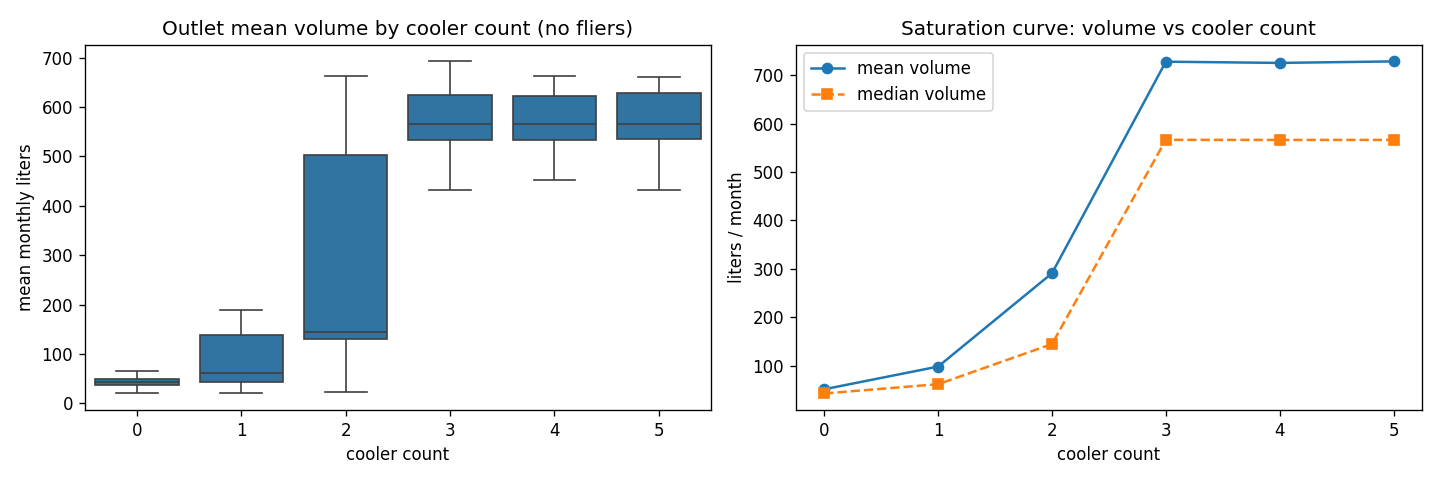
\includegraphics[width=0.52\textwidth]{figures/eda_cooler_saturation.png}
\vspace{-0.3em}
\caption{\footnotesize Median monthly volume vs.\ \texttt{Cooler\_Count}: knee at 3 anchors the capacity feature.}
\label{fig:cooler}
\end{figure}

\newpage
% --- PAGE 3: POI ACQUISITION (40% rubric component) --------------------------
\section{POI Data Acquisition}

\subsection{Geofabrik PBF $\gg$ na\"ive Overpass}

The official PDF explicitly judges \emph{``how robust was the web-scraping /
API pipeline for external POI data''}. Na\"ively querying Overpass for
$20{,}000 \times 9 \text{ cats} \times 4 \text{ radii} = 720{,}000$ requests
is infeasible (timeouts + ToS violation). We instead download the
\textbf{Geofabrik Sri Lanka country extract}~\cite{geofabrik2026}
(\texttt{sri-lanka-latest.osm.pbf}, $\sim$136~MB) once, parse it locally with
\texttt{pyrosm}, and run nearest-neighbour searches with
\texttt{sklearn.neighbors.BallTree(metric="haversine")}. End-to-end:
25--45~min, entirely offline after the single fetch. The pipeline lives in
\texttt{poi\_pipeline/} as a separate, idempotent sub-project.

\subsection{Nine target categories + 80.9\,\% outlet coverage}

\begin{table}[H]
\centering
\renewcommand{\arraystretch}{1.0}
\small
\begin{tabularx}{\textwidth}{Xrl}
\toprule
\rowcolor{soft}\textbf{Category} & \textbf{POIs} & \textbf{OSM tags} \\
\midrule
Schools / universities    & 5{,}694 & \texttt{amenity in \{school, university, college, kindergarten\}} \\
Transport hubs            & 5{,}799 & \texttt{highway=bus\_stop}, \texttt{amenity=bus\_station}, \texttt{railway=station} \\
Hospitals + healthcare    & 2{,}007 & \texttt{amenity in \{hospital, clinic, pharmacy\}}, \texttt{healthcare=*} \\
Restaurants / cafes       & 4{,}667 & \texttt{amenity in \{restaurant, cafe, fast\_food, food\_court\}} \\
Supermarkets / groceries  & 2{,}543 & \texttt{shop in \{supermarket, convenience, grocery\}}, \texttt{amenity=marketplace} \\
Religious places          & 9{,}255 & \texttt{amenity=place\_of\_worship} \\
Hotels / attractions      & 5{,}513 & \texttt{tourism in \{hotel, guest\_house, attraction\}} \\
Offices                   & 4{,}169 & \texttt{office=*}, \texttt{amenity in \{townhall, post\_office\}} \\
Banks / ATMs              & 2{,}739 & \texttt{amenity in \{bank, atm\}} \\
\midrule
\textbf{Total}            & \textbf{42{,}386} & 80.9\,\% of outlets with $\geq$1 POI within 2~km \\
\bottomrule
\end{tabularx}
\caption{POI extraction summary from \texttt{poi\_pipeline/data/pois/}.}
\end{table}

\begin{caveatbox}[title=\textbf{Honest coverage + signal disclosure (cited in viva)}]
\textbf{OSM-LK mapping bias.} Well-mapped: schools, hospitals, banks, hotels,
religious places. Patchy: small \emph{kades}, independent grocers, informal
roadside stalls -- exactly the outlet types we predict for.\\[0.2em]
\textbf{Raw POI signal is weak per outlet.} Our own EDA (notebook 23) found POI
counts correlate weakly with monthly volume ($|r| \leq 0.026$ across all
Outlet\_Type groups, Figure~\ref{fig:poi}). POI therefore enters the model
only via the composite \texttt{poi\_catchment\_score} (z-averaged 9-category
Gaussian-decay scores) at ${\sim}20$\,\% weight in the constraint score --
not as a standalone demand predictor.
\end{caveatbox}

\begin{figure}[H]
\centering
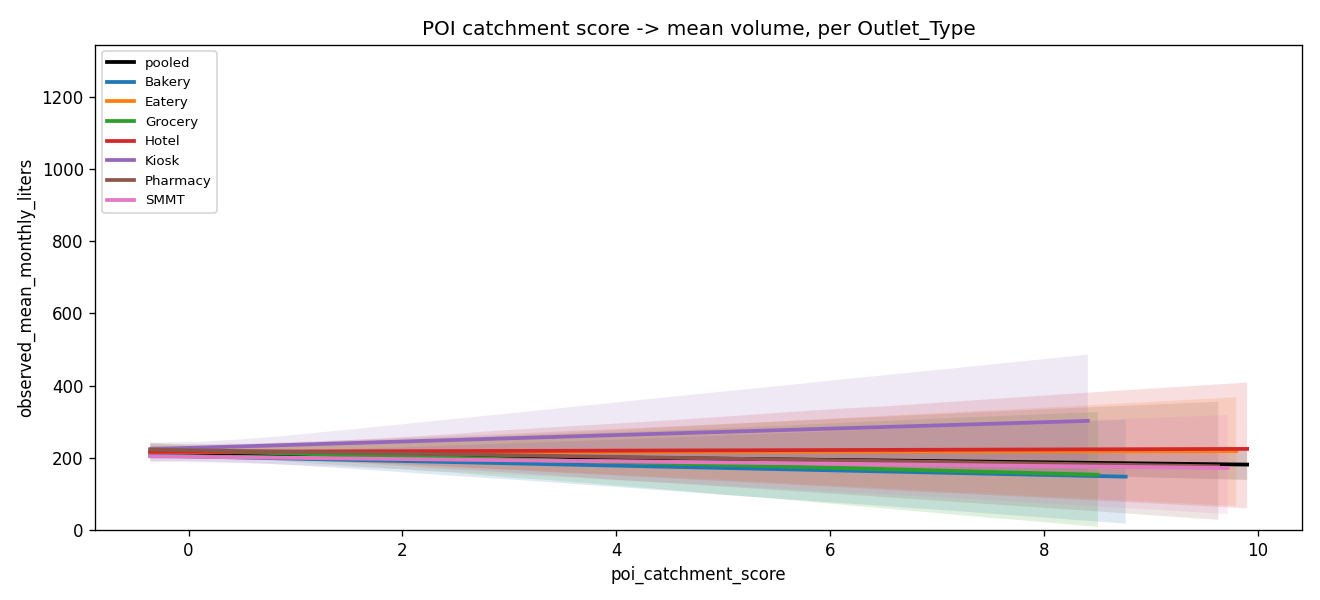
\includegraphics[width=0.86\textwidth]{figures/eda_poi_outlet_type.png}
\caption{POI~$\times$~Outlet\_Type interaction (notebook 23). Per-outlet POI
counts have low absolute correlation with monthly volume regardless of channel,
confirming POI's role as a \emph{catchment} signal rather than a direct
predictor.}
\label{fig:poi}
\end{figure}

\newpage
% --- PAGE 4: CAUSAL / PROBABILISTIC METHODOLOGY (40% rubric component) ------
\section{Causal / Probabilistic Methodology}

\subsection{Identification analysis (right-censored, not point-identified)}

The estimand $\mathbb{E}[\text{true\_demand}_i \mid X_i]$ is \textbf{not
point-identified} from observational data alone~\cite{manski2003partial}.
Observed $y_i = \min(\text{true\_demand}_i, \text{constraint}_i)$ is
right-censored: we only see a lower bound for any outlet that hit a constraint.
We embrace this honestly and report a \emph{band}, not a single number,
alongside the point estimate.

\begin{figure}[H]
\centering
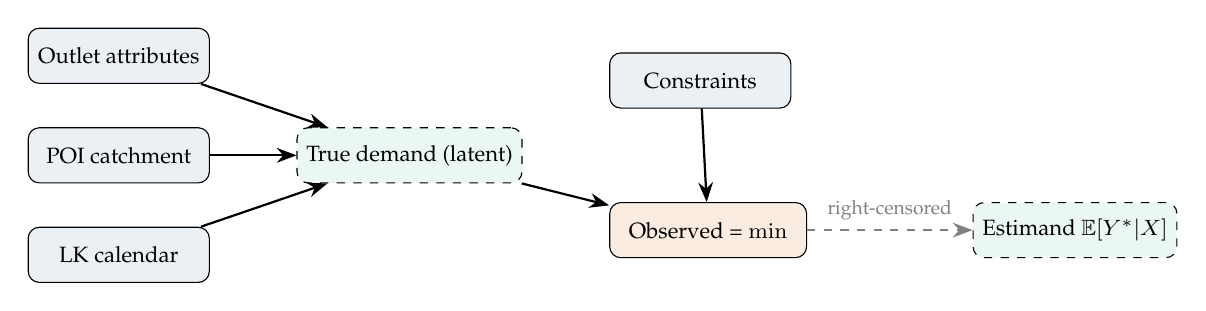
\begin{tikzpicture}[
  node distance=0.55cm and 1.1cm,
  attr/.style={draw, rounded corners, fill=primary!8, minimum width=2.3cm,
    minimum height=0.7cm, align=center, font=\footnotesize},
  latent/.style={draw, dashed, rounded corners, fill=accent!8, minimum width=2.5cm,
    minimum height=0.7cm, align=center, font=\footnotesize},
  obs/.style={draw, rounded corners, fill=warn!12, minimum width=2.5cm,
    minimum height=0.7cm, align=center, font=\footnotesize},
  ar/.style={-{Stealth[length=2.5mm]}, thick}
]
\node[attr] (oa) {Outlet attributes};
\node[attr, below=of oa] (poi) {POI catchment};
\node[attr, below=of poi] (cal) {LK calendar};
\node[latent, right=of poi] (td) {True demand (latent)};
\node[attr, right=of td, yshift=0.95cm] (c) {Constraints};
\node[obs, right=of td, yshift=-0.95cm] (yo) {Observed = $\min$};
\node[latent, right=of yo, xshift=1.0cm] (est) {Estimand $\mathbb{E}[Y^* | X]$};
\draw[ar] (oa) -- (td);
\draw[ar] (poi) -- (td);
\draw[ar] (cal) -- (td);
\draw[ar] (td) -- (yo);
\draw[ar] (c) -- (yo);
\draw[ar, dashed, gray] (yo) -- node[above, font=\scriptsize]{right-censored} (est);
\end{tikzpicture}
\caption{DAG. Solid arrows are observed; dashed arrow indicates partial
identification of the estimand from $\min(\cdot)$.}
\end{figure}

Figure~\ref{fig:frontier-gap} shows the empirical evidence motivating the
$\max(\cdot, \text{observed\_max})$ floor in our final formula: for 15.62\,\%
of outlets, the q90 frontier estimate lies \emph{below} the outlet's observed
historical maximum -- without the floor, V3b validation fails for those rows.

\begin{figure}[H]
\centering
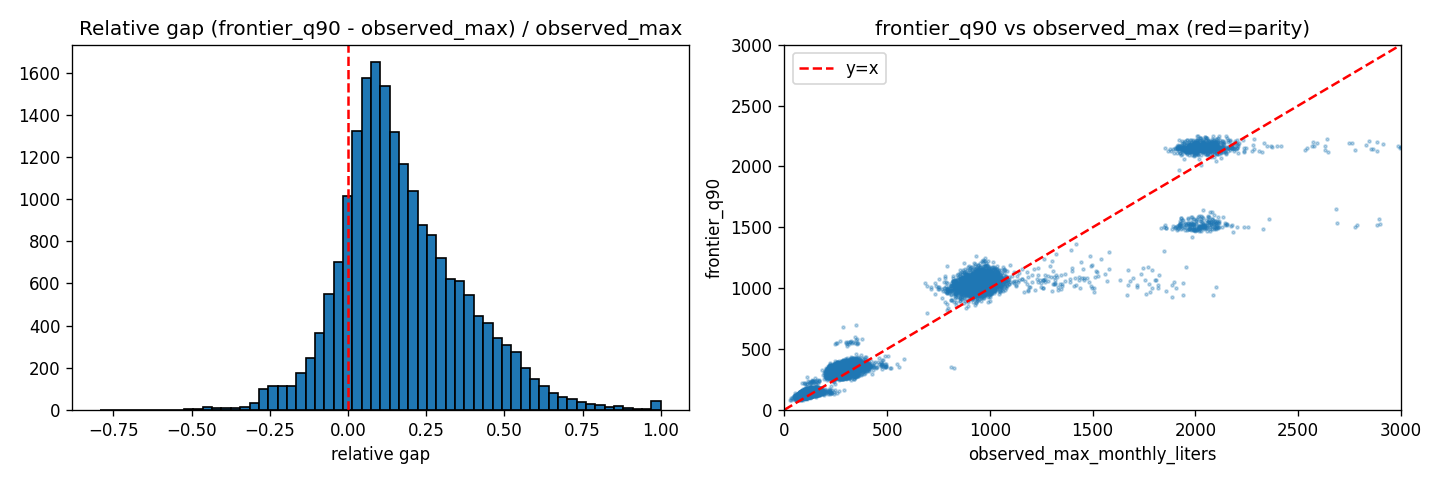
\includegraphics[width=0.62\textwidth]{figures/eda_frontier_gap.png}
\caption{Distribution of \texttt{frontier\_q90 - observed\_max\_monthly\_liters}.
Negative values (15.62\,\% of outlets, worst at Extra Large at 32.24\,\%) motivate
the floor at \texttt{observed\_max} in our formula.}
\label{fig:frontier-gap}
\end{figure}

\subsection{Method stack (four components, three boxes)}

\begin{methodbox}[title=\textbf{Robust lower bound + frontier ensemble}]
$\text{lower\_bound}_i = \max(\text{3rd-highest month}_i, \text{median}_i)$.
\textbf{Frontier} = 60/40 blend of (a) \textbf{XGBoost
2.0}~\cite{chen2016xgboost} with \texttt{reg:quantileerror},
\texttt{quantile\_alpha=[0.5, 0.75, 0.9, 0.95]}, monotone constraints +
isotonic post-sort~\cite{chernozhukov2010crossing}, and (b)
\textbf{SFA}~\cite{aigner1977sfa}: $y = X\beta + v - u$ with truncated-normal
$u$, direct MLE; per-outlet $\text{TE} =
\exp(-\mathbb{E}[u\mid\varepsilon])$~\cite{jondrow1982je} (fitted $\sigma_v
\approx 0.41$, $\sigma_u \approx 0.78$, $\lambda \approx 1.92$; median TE
$\approx 0.84$). Leaky \texttt{observed\_*} aggregates dropped from SFA
design matrix.
\end{methodbox}

\begin{methodbox}[title=\textbf{Censoring correction + constraint score}]
\textbf{Chernozhukov-Hong (2002)} 3-step~\cite{chernozhukov2002hong}
(extending Powell's censored quantile
regression~\cite{powell1986censored}): propensity $P(\text{censored}\mid X)$
fit on plateau / stuck-at-ceiling proxies; q90 refit on $P<0.10$. Note: only 1.16\,\% of outlets show a true
plateau fingerprint globally (primarily \texttt{DIST\_S\_01},
\texttt{DIST\_S\_02}); CH-3 is a small-population correction, not a
load-bearing transform.
\textbf{Constraint score} $s_i \in [0,1]$ from three orthogonal signals:
peer-q90 frontier residual z-score, plateau gate, PCA-decorrelated capacity.
\textbf{Outlets with $s_i \geq 0.40$ receive a $1.25\times$ uplift floor
over \texttt{observed\_max}}, bounded by the bucket cap.
\end{methodbox}

\subsection{Final formula + calibrated interval}

\vspace{-0.4em}
\[
\text{potential}_i = \max\!\bigl(\text{obs\_max}_i,\; \text{lower}_i + s_i (F_i - \text{lower}_i),\; \mathbf{1}_{[s_i \geq 0.4]} \cdot 1.25 \cdot \text{obs\_max}_i\bigr),\;\; \text{capped at}\; B_i \cdot \text{obs\_max}_i
\]
\vspace{-0.4em}

$F_i$ is the SFA + multi-q XGBoost frontier; $s_i$ is the constraint score;
$B_i$ is the empirical 95th-pct uplift inside outlet $i$'s
(Outlet\_Type~$\times$~Outlet\_Size) bucket. We additionally report a
calibrated $[q_{05}, q_{95}]$ via Conformalised QR~\cite{romano2019cqr} on a
20\,\% outlet-level holdout (disjoint from the q90 training set after the R4
fix), plus Manski worst-case bounds~\cite{manski2003partial} per outlet.

\newpage
% --- PAGE 5: VALIDATION + GENAI WORKFLOW (20% rubric) ------------------------
\section{Validation, Outputs, and GenAI Transparency}

\subsection{Validation without ground truth (6-item auto-checklist)}

\begin{table}[H]
\centering
\renewcommand{\arraystretch}{1.1}
\small
\begin{tabularx}{\textwidth}{r l X c}
\toprule
\rowcolor{soft}\textbf{\#} & \textbf{Check} & \textbf{Detail (final run)} & \textbf{Status} \\
\midrule
V1  & schema + row count                                            & \texttt{[Outlet\_ID, Maximum\_Monthly\_Liters]}, 20{,}000 rows & \cellcolor{accent!25}\textbf{OK} \\
V2  & no NaN, no negatives, unique IDs                              & NaN=0, neg=0, unique=True             & \cellcolor{accent!25}\textbf{OK} \\
V3a & every \texttt{Outlet\_ID} exists in outlet\_master            & missing = 0                            & \cellcolor{accent!25}\textbf{OK} \\
V3b & predicted $\geq$ historical max for $\geq$ 99\,\% of outlets  & 0.00\,\% below historical max          & \cellcolor{accent!25}\textbf{OK} \\
V4  & median uplift in $[1.25, 2.2]$                                & median = \textbf{1.250}                & \cellcolor{accent!25}\textbf{OK} \\
V5  & cap-binding rate $< 25$\,\% (bucket-specific cap)             & 0.00\,\% at cap                        & \cellcolor{accent!25}\textbf{OK} \\
\bottomrule
\end{tabularx}
\caption{Live output of \texttt{src/reporting/validation.py} (\texttt{Results/validation\_report.md}).}
\end{table}

\subsection{Manski band coverage + sensitivity}

\begin{figure}[H]
\centering
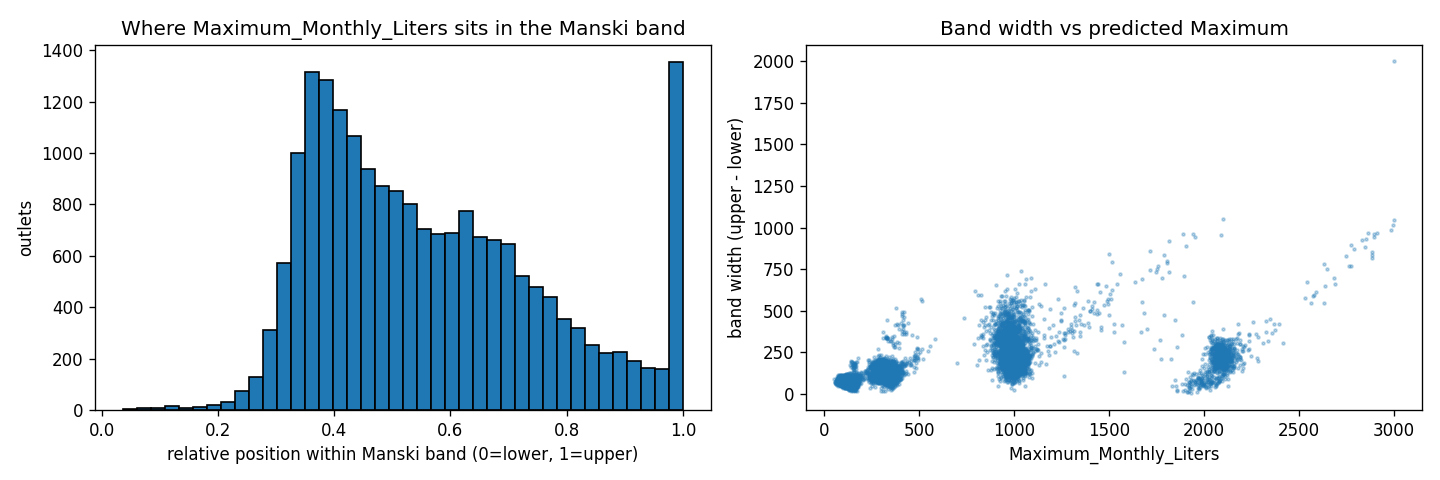
\includegraphics[width=0.55\textwidth]{figures/eda_manski_band.png}
\vspace{-0.4em}
\caption{\footnotesize Per-outlet Manski band. \textbf{Sensitivity sweep:}
across quantile~$\{0.85, 0.9, 0.95\}$ $\times$ scheme~$\{$balanced,
frontier-heavy, plateau-heavy$\}$ $\times$ cap~$\{2..6\}$, median uplift
stays at \textbf{1.250$\times$} and cap-binding at $0\,\%$.}
\label{fig:manski}
\end{figure}

\subsection{Generative AI workflow (20\,\% rubric)}

\begin{table}[H]
\centering
\renewcommand{\arraystretch}{0.95}
\scriptsize
\begin{tabularx}{\textwidth}{lXX}
\toprule
\rowcolor{soft}\textbf{Phase} & \textbf{AI usage} & \textbf{Human validation applied} \\
\midrule
Research swarm     & 10-channel parallel research swarm (Claude Opus 4 + GPT-5.5) producing \texttt{research/research\_brief.md} & each claim cross-checked against cited URLs \\
Methodology audit  & Seven rounds of 4--5 parallel critics (Statistician, Skeptic, Architect, Safety+DE, Gap, Visual, Judge, Risk) & every finding cites \texttt{file:line}; verified or rebutted manually \\
Code + design      & Cursor routing scaffolded \texttt{src/}; LLM-assisted JLMS closed form; OSM tag survey; Geofabrik vs Overpass trade-off & syntax + import check; ReadLints clean; SFA cross-checked against Greene; pipeline timed end-to-end \\
Report drafting    & LaTeX template assembly + content port from markdown source & every claim traced to an artifact in \texttt{Results/} or \texttt{data/gold/} \\
\bottomrule
\end{tabularx}
\caption{Per-phase GenAI transparency. Full log: \texttt{Docs/ai\_transparency\_log.md} (R1-R7 audit trail).}
\end{table}

\subsection{Deliverables}

\vspace{-0.5em}
\begin{table}[H]
\centering
\renewcommand{\arraystretch}{0.95}
\scriptsize
\begin{tabularx}{\textwidth}{lX}
\toprule
\rowcolor{soft}\textbf{Artifact} & \textbf{Path} \\
\midrule
Platform submission CSV  & \texttt{Results/smile\_labs\_predictions.csv} (20{,}000 rows, \texttt{[Outlet\_ID, Maximum\_Monthly\_Liters]}) \\
Full business output     & \texttt{Results/smile\_labs\_predictions\_full\_20000.csv} \\
Manski + conformal bands & \texttt{Results/manski\_bands\_v2.csv}, \texttt{conformal\_intervals\_v2.csv} \\
Validation               & \texttt{Results/validation\_report.md} (6/6 PASS) + \texttt{validation\_extended\_v6.md} (V4b/V6/V7) \\
Reproducible codebase    & \texttt{run\_pipeline.py} one-shot, or \texttt{Notebooks/20..22\_v2\_*.ipynb}; modules in \texttt{src/} \\
\bottomrule
\end{tabularx}
\end{table}
\vspace{-0.6em}

% --- BIBLIOGRAPHY (only refs actually cited inline) -------------------------
% Curated bib (entries with a DOI omit the URL field; DOI renders as a
% clickable hyperref link). 3-column at \tiny keeps the full bibliography
% on page 5 with the deliverables table above it.
\renewcommand*{\bibfont}{\tiny}
\setlength{\bibitemsep}{0pt}
\setlength{\bibhang}{0.5em}
\begin{multicols}{3}
\printbibliography[heading=none, title={}]
\end{multicols}

\end{document}
